\section{OOP}



\subsection{Question - 2 points}



\subsubsection{Expliquez ce qu'est l'overloading}
\color[rgb]{0,0.48,0.58}
C'est le fait de d'implémenter deux méthodes de même nom mais de signature différente (paramètres différents).
\\Exemple:
\begin{itemize}
    \item bool maFonction( val1 );
	\item bool maFonction( val1, val2 );
\end{itemize}
\color[rgb]{0,0,0}



\subsubsection{Expliquez ce qu'est l'overriding}
\textcolor[rgb]{0,0.48,0.58}{C'est le fait de re-implémenter une méthode fille qui a déjà été implémenté dans sa classe parente, et donc de remplacer l'appel de l'ancienne méthode par la nouvelle. On peut appeler la méthode parente en appliquant super.NomDeLaMethode(...) }



\subsubsection{Expliquez l'utilité de ces deux concepts}
\textcolor[rgb]{0,0.48,0.58}{L'overloading et l'overriding sont, chacune, une des particularités du polymorphisme. On peut par exemple imaginer surcharger les opérateurs +,-,*, ... pour divers classes avec l'overloading ou modifier une méthode d'une classe parente dans la classe fille.}



\subsection{Question - 2 points}



\subsubsection{Définissez le concept de polymorphisme}
\textcolor[rgb]{0,0.48,0.58}{Polymorphisme: On envoie un même message à des objets de forme différente et la réponse pourra être différente.}



\subsubsection{Expliquez l'utilité du polymorphisme dans les langages orienté objet}
\textcolor[rgb]{0,0.48,0.58}{Le polymorphisme est utile dans le cas où l'on a plusieurs sous classes qui héritent d'une classe virtuelle (virtuelle pure). Les méthodes de ces sous classes peuvent être redéfinies (doivent être dans le cas d'une virtuelle pure). Lorsqu'un message est envoyé, et suivant la redéfinition de la classe, le résultat ne sera pas le même.}



\subsection{Question - 2 points}
Étant donné le diagramme de classes suivant et que les méthodes sont définies de la façon suivante :
\begin{itemize}
	\item A - M1() : Print "A-M1"
	\item B - M2() : Super M1()
    \item B - M3() : Self M1()
	\item C - M1() : Print "C-M1"
\end{itemize}
\begin{figure}[h]
	\centering
		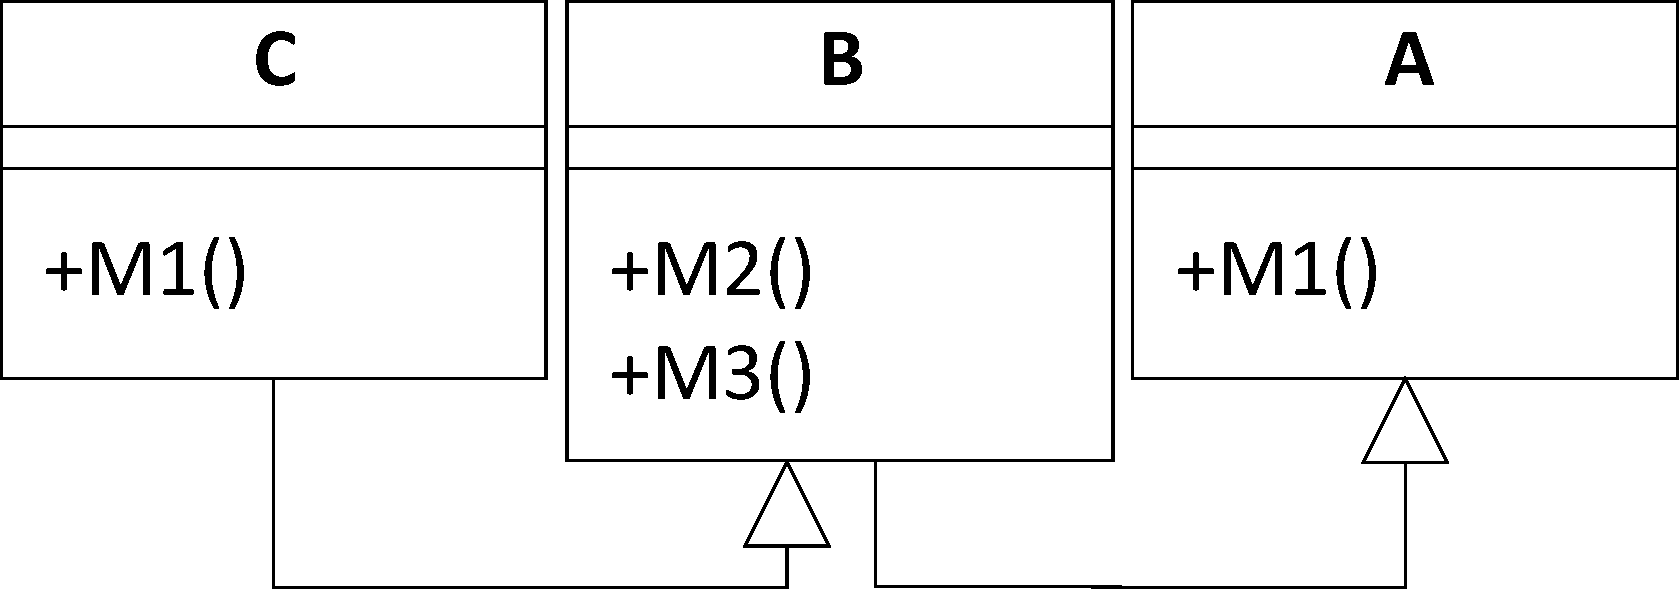
\includegraphics[width=0.50\textwidth]{questions-reponses/2.oop/DiaDeClasse0.pdf}
	\label{fig:DiaDeClasse0}
\end{figure}



\subsubsection{Sachant que a est une référence vers la classe A, b est une référence vers la classe B et c une référence vers la classe C, identifiez les assignations qui sont valides}
\begin{enumerate}[a)]
	\item \textbf{a = b} \textcolor[rgb]{0,0.48,0.58}{Valide}
	\item \textbf{b = a} \textcolor[rgb]{0,0.48,0.58}{Erreur, c'est \textbf{b} qui hérite de \textbf{a}. Donc \textbf{b} est une sorte de \textbf{a} et pas l'inverse. (Exemple: Une \textbf{b}aleine est un \textbf{a}nimal, mais un \textbf{a}nimal n'est pas forcément une \textbf{b}aleine. L'\textbf{a}nimal pourrait être autre chose...)}
	\item \textbf{b = c} \textcolor[rgb]{0,0.48,0.58}{Valide}
	\item \textbf{A al = new C} \textcolor[rgb]{0,0.48,0.58}{Erreur, A al = C mais une référence n'enregistre pas une adresse (new).}
\end{enumerate}



\subsubsection{Déterminez ce qui est affiché lors des appels ci-dessous si a2 est une référence de classe B référençant un objet de classe C}
\begin{enumerate}[a)]
	\item \textbf{a2.M2()} \textcolor[rgb]{0,0.48,0.58}{B.M2() $\rightarrow$ A.M1() $\rightarrow$ Print "A-M1"}
	\item \textbf{a2.M3()} \textcolor[rgb]{0,0.48,0.58}{B.M3() $\rightarrow$ C.M1() $\rightarrow$ Print "C-M1"}
\end{enumerate}



\subsection{Question - 2 points}
Étant donné le diagramme de classes suivant et que b et c référencent respectivement des objets des classes B et C :
\begin{figure}[ht]
	\centering
		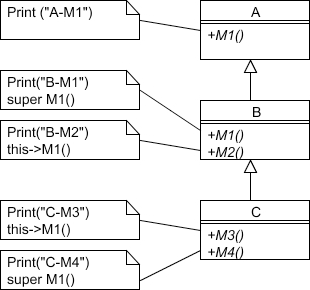
\includegraphics[height=0.50\textwidth]{questions-reponses/2.oop/DiaDeClasse.png}
	\label{fig:DiaDeClasse}
\end{figure}



\subsubsection{Déterminez ce qui est affiché lors des appels}
\begin{enumerate}[a)]
	\item \textbf{b.M1()} \textcolor[rgb]{0,0.48,0.58}{B-M1 / A-M1}
	\item \textbf{b.M2()} \textcolor[rgb]{0,0.48,0.58}{B-M2 / B-M1 / A-M1}
	\item \textbf{c.M3()} \textcolor[rgb]{0,0.48,0.58}{C-M3 / B-M1 / A-M1}
	\item \textbf{c.M4()} \textcolor[rgb]{0,0.48,0.58}{C-M4 / B-M1 / A-M1}
\end{enumerate}



\subsubsection{Expliquez la différence entre les méthodes M3 et M4.}
\textcolor[rgb]{0,0.48,0.58}{Dans le cas de M3, on appelle la méthode M1 sur l'objet lui-même (sur C), comme M1 n'existe pas, on va voir dans la classe parente qui est B.
\\Dans le cas de M4, on appelle directement la méthode de la classe parente (B).
\\Ici, il n'y a pas de différence étant donné que la méthode M1 n'existe pas dans la classe C ; on va donc voir dans les deux cas dans la classe parente.}



\subsubsection{Illustrez cette différence en étendant le diagramme UML mais sans modifier les éléments déjà existants.}
\textcolor[rgb]{0,0.48,0.58}{En définissant C.M1() et le faisant Print(“C-M1”). Ainsi C.M3() appelera C.M1() et C.M4() appelera B.M1() et on notera la différence.}



\subsection{Question 5 points}



\subsubsection{Définissez et expliquez l'utilité des concepts suivant}

\begin{itemize}
	\item \textbf{Self (this) et Super}
\end{itemize}
\color[rgb]{0,0.48,0.58}
Self (this) référence l'objet courant de la classe.
\\Super référence l'objet parent de l'objet courant de la classe.
\\Utilité : Tout ceci sert pour le polymorphisme. Super peut servir pour redéfinir une méthode parente en l'appelant puis en changeant son résultat. Self est aussi utile pour le polymorphisme puisqu'il permet de s'assurer qu'on appellera la méthode courante si elle existe (Sinon elle se redirigea vers celle du parent).
\color[rgb]{0,0,0}

\begin{itemize}
	\item \textbf{Classe abstraite (Abstract class)}
\end{itemize}
\color[rgb]{0,0.48,0.58}
Une classe est dîtes abstraite quand au moins une de ses méthodes est virtuellement pure. ( type methode() = 0; ) La classe abstraite n'est pas complète et n'est donc pas instanciable seule.
\\Elle sert de base aux classes filles et si la classe fille ne veut pas être abstraite elle doit redéfinir toutes les méthodes virtuelles pures de la mère. Si elle le fait, on appelle ça une concrétisation.
\color[rgb]{0,0,0}


\begin{itemize}
	\item \textbf{Interface}
\end{itemize}
\color[rgb]{0,0.48,0.58}
Le principe d'une interface est donnée par l'utilisation de classe abstraite. Elle fournit une abstraction qui permettra de mettre des choses en commun entre ses filles. Cette classe ne contient que des déclarations de fonctions virtuelles et pas d’attributs, ça permet de rajouter des contraintes d’implémentation.
\color[rgb]{0,0,0}

\begin{itemize}
	\item \textbf{Héritage}
\end{itemize}
\color[rgb]{0,0.48,0.58}
On dérive d’une classe parente et les sous-classes héritent de tous ses attributs et méthode.
Les sous-classes peuvent surcharger les méthode pour les adapter à leurs besoins $\Rightarrow$ Overriding.
\\\textbf{But}: Mettre de la structure qui amènera au polymorphisme et un code facilement maintenable.
Pour savoir si B doit hériter de A, il faut pouvoir se dire : B est une sorte de A.
\\Il exite 2 types d'héritages :
\begin{itemize}
	\item \textbf{Héritage simple} : Une classe hérite d’une seule et une seule classe. Cet héritage à une structure d’arbre, chaque classe a un parent et des enfants.
	\item \textbf{Héritage multiple} : Permet d’hériter directement de plusieurs classe. Les langages récents ne le permettent plus car plus de problème que de solution.
\end{itemize}
\color[rgb]{0,0,0}

\begin{itemize}
	\item \textbf{Polymorphisme}
\end{itemize}
\textcolor[rgb]{0,0.48,0.58}{Polymorphisme: On envoie un même message à des objets de forme différente et la réponse pourra être différente.}